\chapter{The Design of Tufte's Books}
\label{ch:tufte-design}

\newthought{The pages} of a book are usually divided into three major sections: the front matter (also called preliminary matter or prelim), the main matter (the core text of the book), and the back matter (or end matter).

\newthought{The front matter} of a book refers to all of the material that comes before the main text. The following table shows a list of material that appears in the front matter of \VDQI, \EI, \VE, and \BE along with its page number. Page numbers that appear in parentheses refer to folios that do not have a printed page number (but they are still counted in the page number sequence).

\bigskip
\begin{minipage}{\textwidth}
\begin{center}
\begin{tabular}{lcccc}
\toprule
& \multicolumn{4}{c}{Books} \\
\cmidrule(l){2-5} 
Page content & \vdqi & \ei & \ve & \be \\
\midrule
Blank half title page & \hangp{1} & \hangp{1} & \hangp{1} & \hangp{1} \\
Frontispiece\footnotemark{}
& \hangp{2} & \hangp{2} & \hangp{2} & \hangp{2} \\
Full title page & \hangp{3} & \hangp{3} & \hangp{3} & \hangp{3} \\
Copyright page & \hangp{4} & \hangp{4} & \hangp{4} & \hangp{4} \\
Contents & \hangp{5} & \hangp{5} & \hangp{5} & \hangp{5} \\
Dedication & \hangp{6} & \hangp{7} & \hangp{7} & 7 \\
Epigraph & -- & -- & \hangp{8} & -- \\
Introduction & \hangp{7} & \hangp{9} & \hangp{9} & 9 \\
\bottomrule
\end{tabular}
\end{center}
\end{minipage}
\vspace{-7\baselineskip}\footnotetext{The contents of this page vary from book to book. In \vdqi this page is blank; in \ei and \ve this page holds a frontispiece; and in \be this page contains three epigraphs.}
\vspace{7\baselineskip}

\bigskip
The design of the front matter in Tufte's books varies slightly from the traditional design of front matter. First, the pages in front matter are traditionally numbered with lowercase roman numerals (\eg, i, ii, iii, iv,~\ldots). Second, the front matter page numbering sequence is usually separate from the main matter page numbering. That is, the page numbers restart at 1 when the main matter begins. In contrast, Tufte has enumerated his pages with arabic numerals that share the same page counting sequence as the main matter.

There are also some variations in design across Tufte's four books. The page opposite the full title page (labeled ``frontispiece'' in the above table) has different content in each of the books. In \VDQI, this page is blank; in \EI and \VE, this page holds a frontispiece; and in \BE, this page contains three epigraphs.

The dedication appears on page~6 in \vdqi (opposite the introduction), and is placed on its own spread in the other books. In \ve, an epigraph shares the spread with the opening page of the introduction.

None of the page numbers (folios) of the front matter are expressed except in \be, where the folios start to appear on the dedication page.

\newthought{The full title page} of each of the books varies slightly in design. In all the books, the author's name appears at the top of the page, the title it set just above the center line, and the publisher is printed along the bottom margin. Some of the differences are outlined in the following table.

\bigskip
\begin{center}
\footnotesize
\begin{tabular}{lllll}
\toprule
Feature & \vdqi & \ei & \ve & \be \\
\midrule
Author & & & & \\
\quad Typeface & serif & serif & serif & sans serif \\
\quad Style & italics & italics & italics & upright, caps \\
\quad Size & 24 pt & 20 pt & 20 pt & 20 pt \\
\addlinespace
Title & & & & \\
\quad Typeface & serif & serif & serif & sans serif \\
\quad Style & upright & italics & upright & upright, caps \\
\quad Size & 36 pt & 48 pt & 48 pt & 36 pt \\
\addlinespace
Subtitle & & & & \\
\quad Typeface & \na & \na & serif & \na \\
\quad Style & \na & \na & upright & \na \\
\quad Size & \na & \na & 20 pt & \na \\
\addlinespace
Edition & & & & \\
\quad Typeface & sans serif & \na & \na & \na \\
\quad Style & upright, caps & \na & \na & \na \\
\quad Size & 14 pt & \na & \na & \na \\
\addlinespace
Publisher & & & & \\
\quad Typeface & serif & serif & serif & sans serif \\
\quad Style & italics & italics & italics & upright, caps \\
\quad Size & 14 pt & 14 pt & 14 pt & 14 pt \\
\bottomrule
\end{tabular}
\end{center}

\begin{figure*}[p]
\fbox{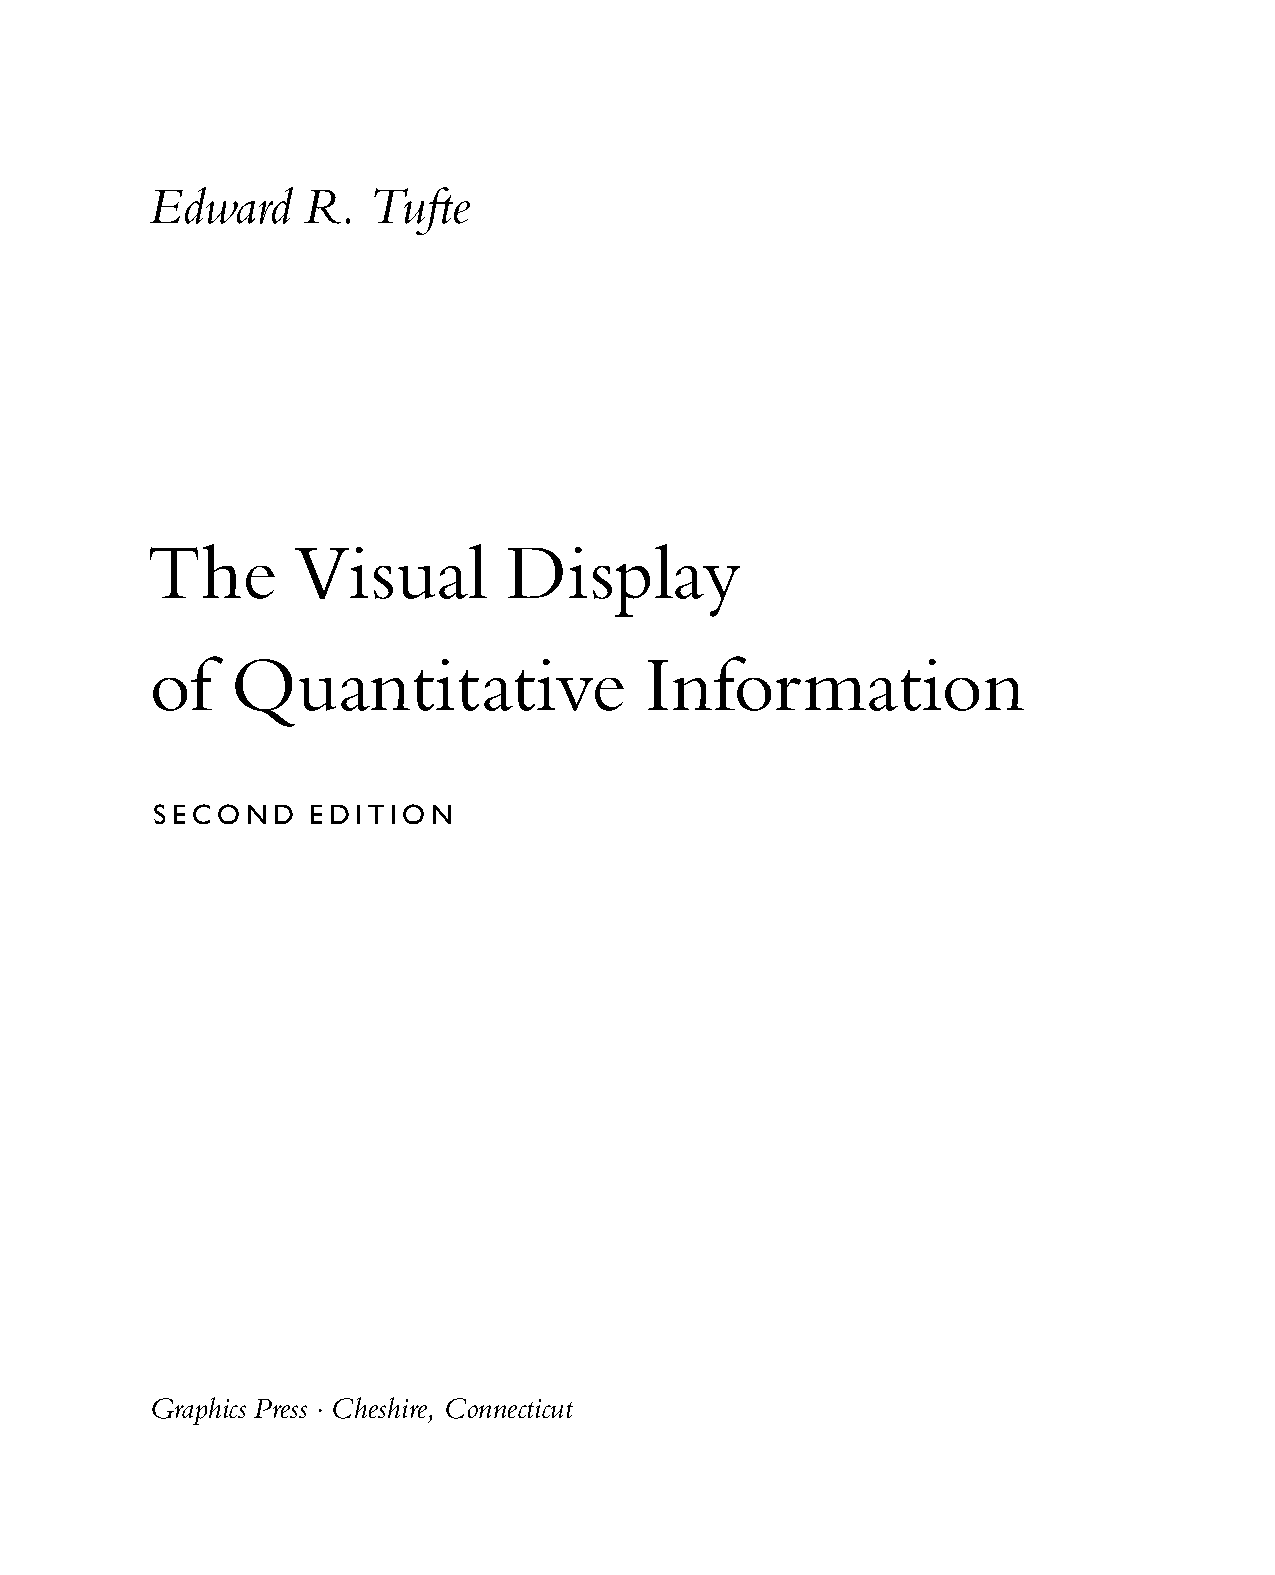
\includegraphics[width=0.45\linewidth]{graphics/vdqi-title.pdf}}
\hfill
\fbox{
\includegraphics[width=0.45\linewidth]{graphics/ei-title.pdf}}
\\\vspace{\baselineskip}
\fbox{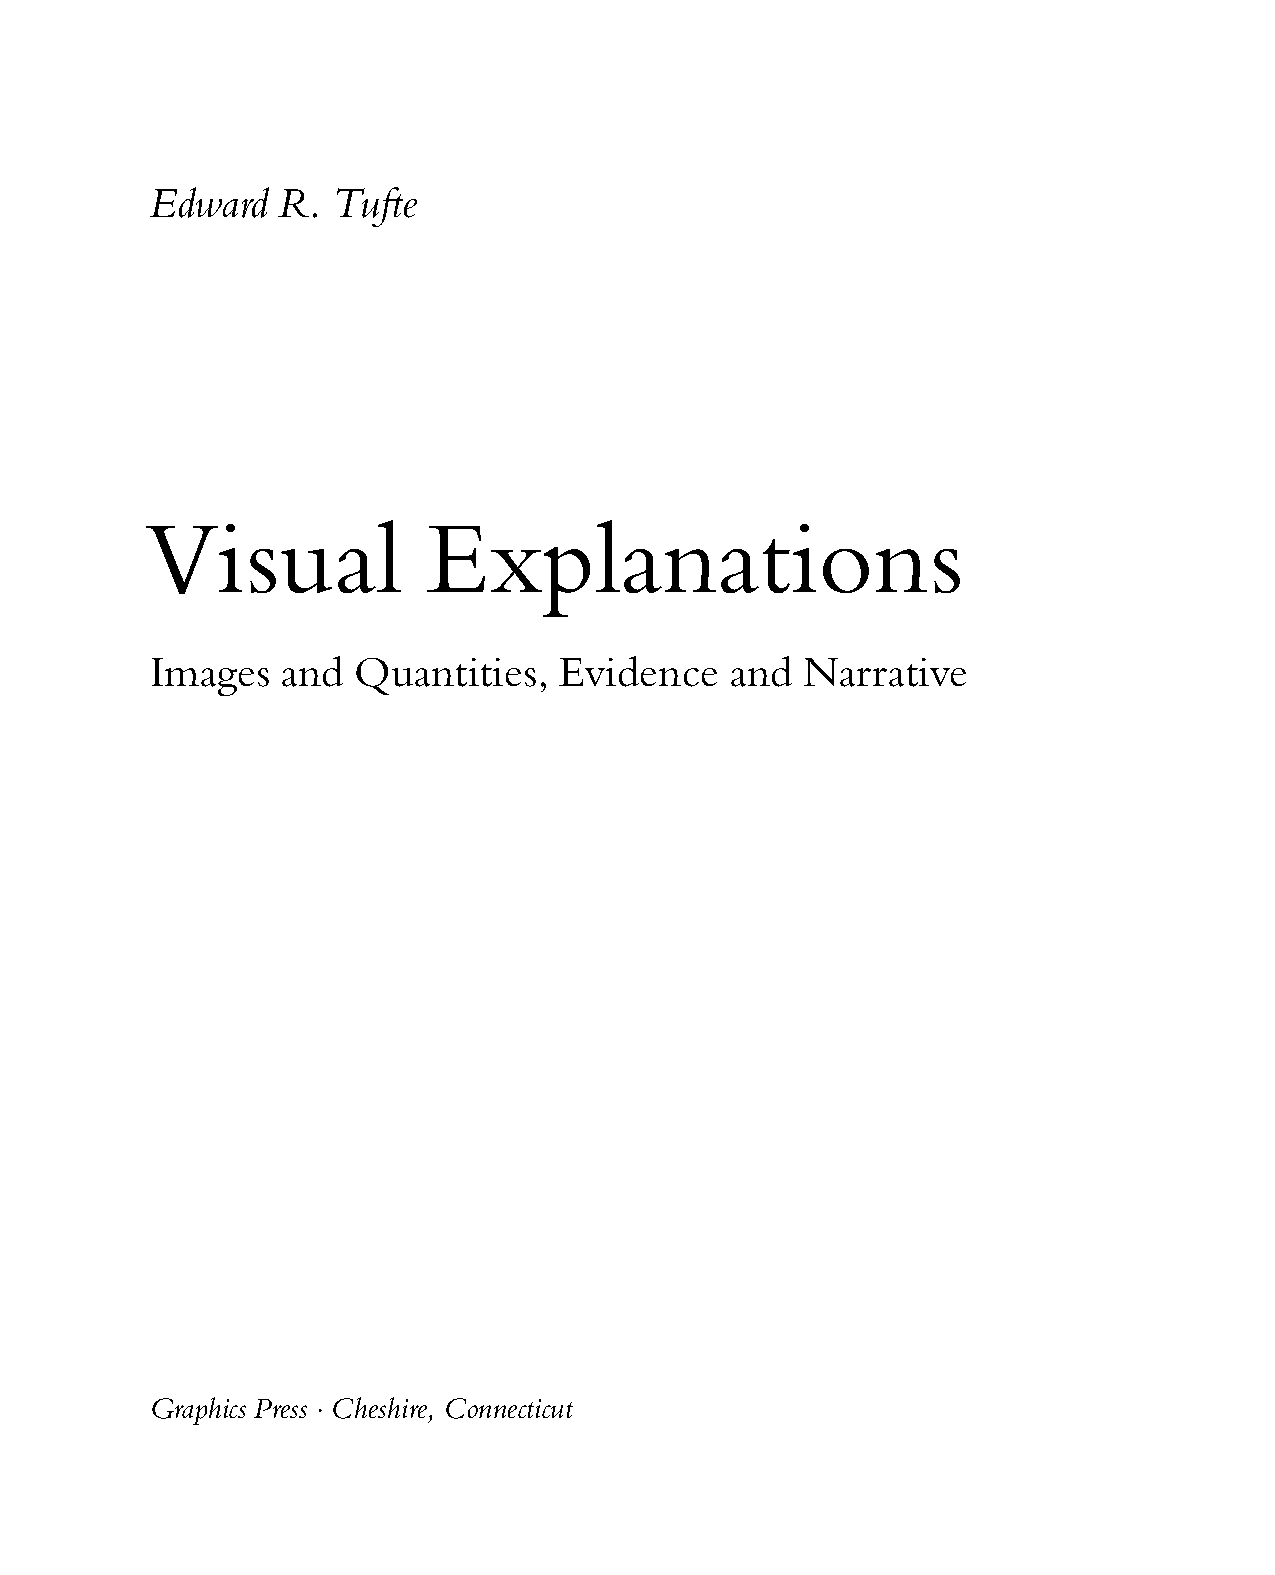
\includegraphics[width=0.45\linewidth]{graphics/ve-title.pdf}}
\hfill
\fbox{
\includegraphics[width=0.45\linewidth]{graphics/be-title.pdf}}
\end{figure*}

\newthought{The tables of contents} in Tufte's books give us our first glimpse of the structure of the main matter. \VDQI is split into two parts, each containing some number of chapters. His other three books only contain chapters---they're not broken into parts.

\begin{figure*}[p]\index{table of contents}
\fbox{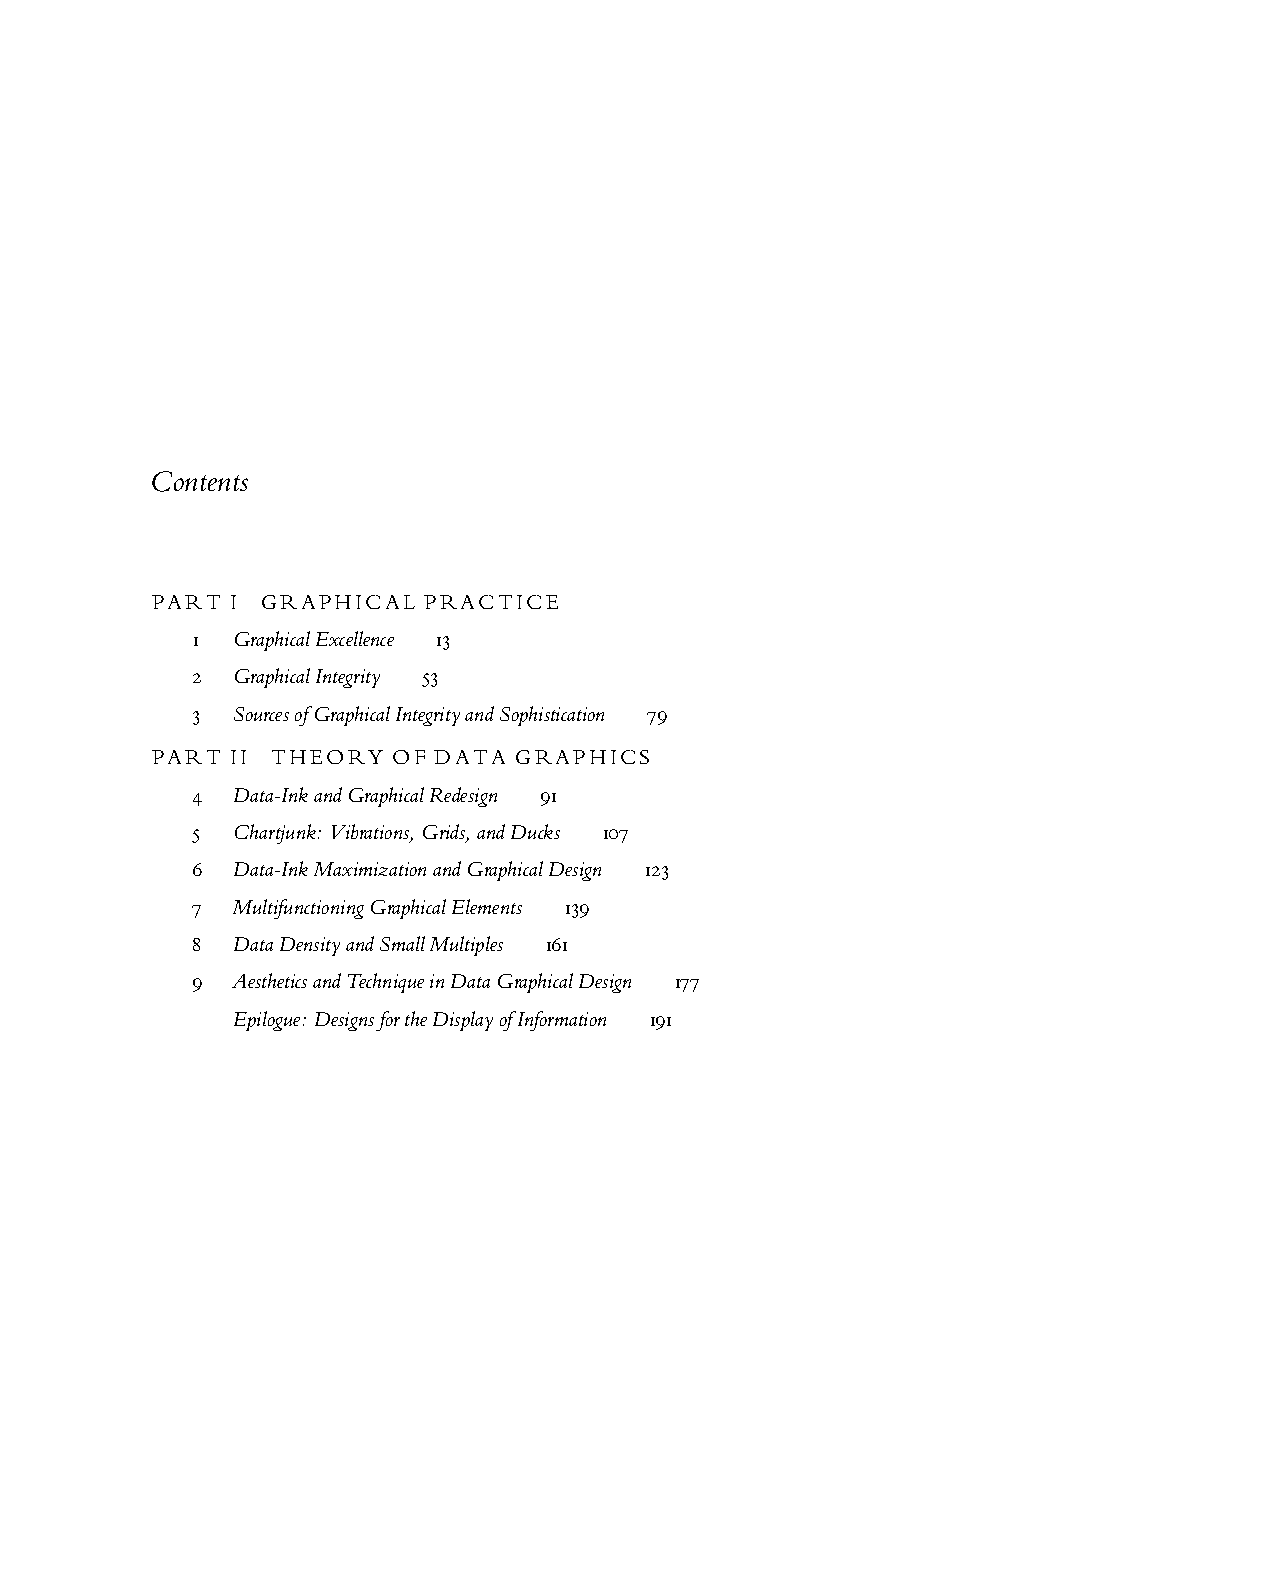
\includegraphics[width=0.45\linewidth]{graphics/vdqi-contents.pdf}}
\hfill
\fbox{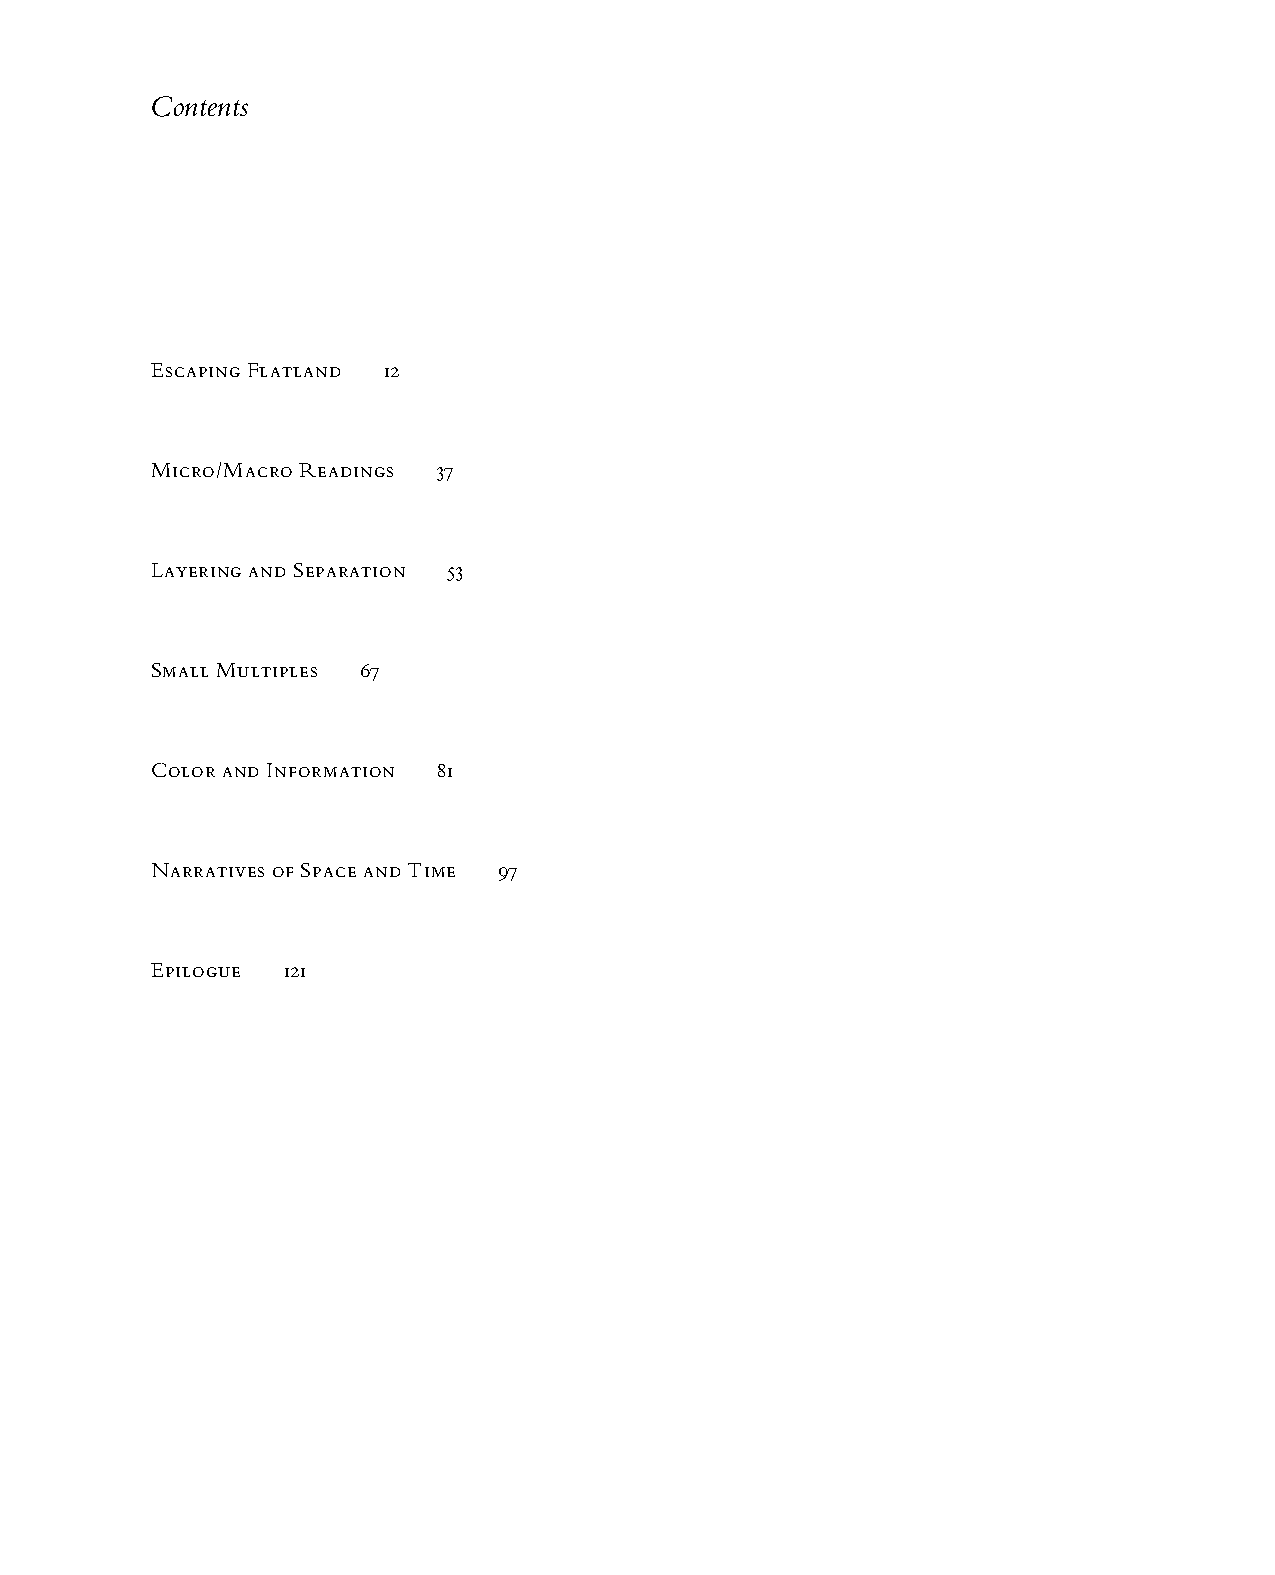
\includegraphics[width=0.45\linewidth]{graphics/ei-contents.pdf}}
\\\vspace{\baselineskip}
\fbox{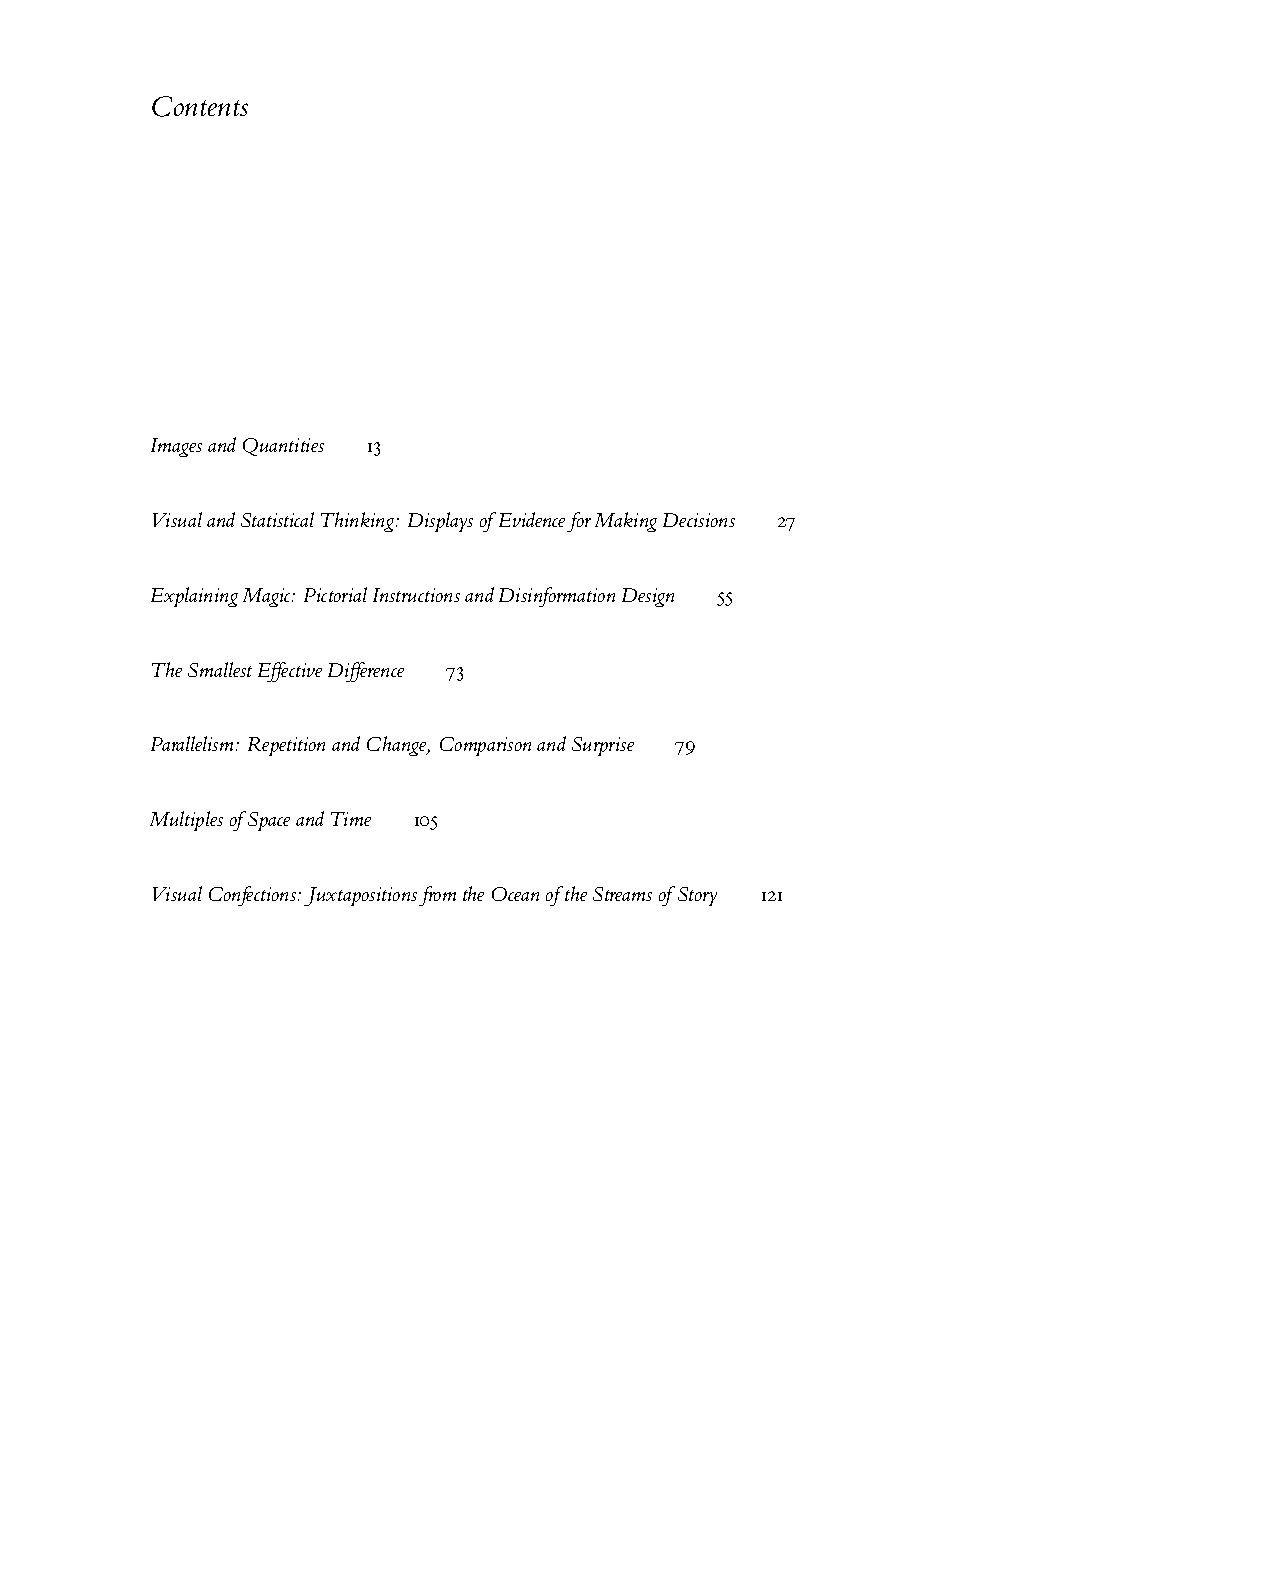
\includegraphics[width=0.45\linewidth]{graphics/ve-contents.pdf}}
\hfill
\fbox{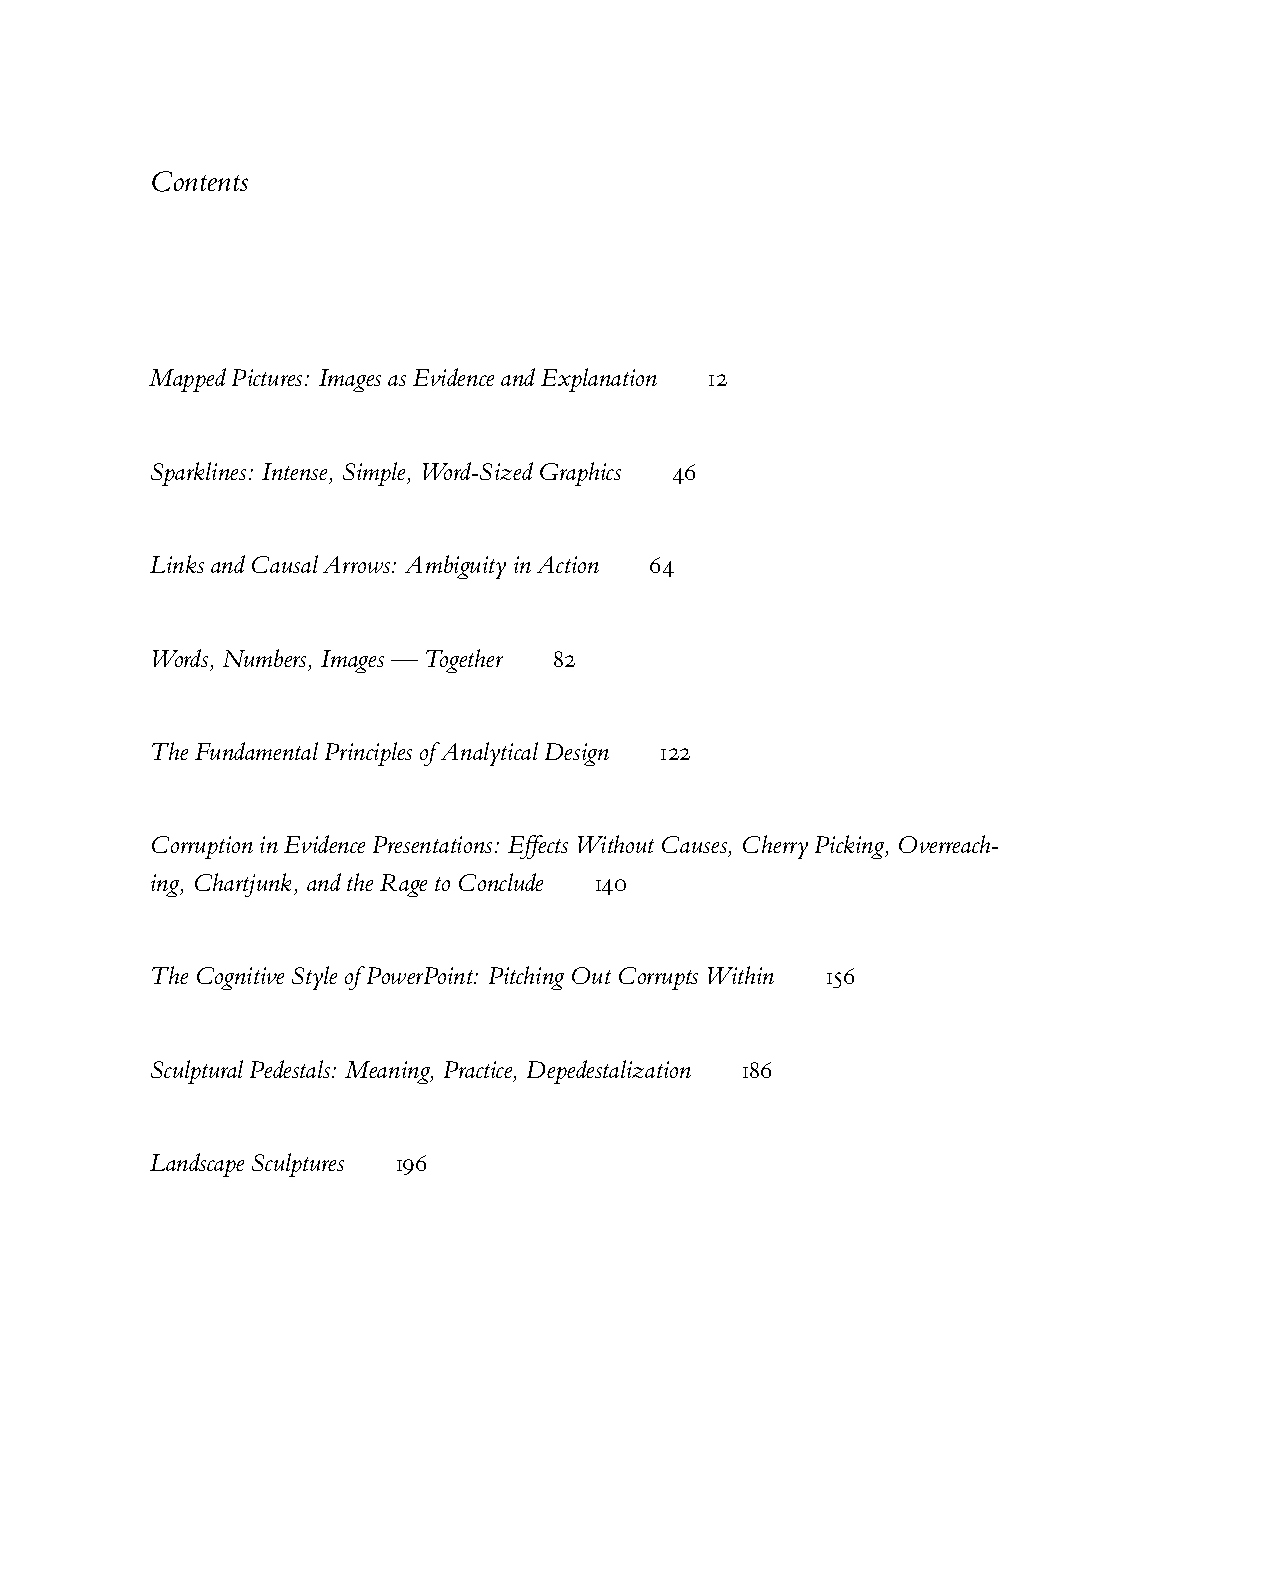
\includegraphics[width=0.45\linewidth]{graphics/be-contents.pdf}}
\end{figure*}

%------------------------------------------------

\section{Typefaces}\label{sec:typefaces1}\index{typefaces}
\index{fonts|see{typefaces}}

Tufte's books primarily use two typefaces: Bembo and Gill Sans. Bembo is used for the headings and body text, while Gill Sans is used for the title page and opening epigraphs in \BE.

Since neither Bembo nor Gill Sans are available in default \LaTeX{} installations, the \TL document classes default to using Palatino and Helvetica, respectively. In addition, the Bera Mono typeface is used for \texttt{monospaced} type.

The following font sizes are defined by the \TL classes:

\begin{table}[h]\index{typefaces!sizes}
\footnotesize%
\begin{center}
\begin{tabular}{lccl}
\toprule
\LaTeX{} size & Font size & Leading & Used for \\
\midrule
\verb+\tiny+ & 5 & 6 & sidenote numbers \\
\verb+\scriptsize+ & 7 & 8 & \na \\
\verb+\footnotesize+ & 8 & 10 & sidenotes, captions \\
\verb+\small+ & 9 & 12 & quote, quotation, and verse environments \\
\verb+\normalsize+ & 10 & 14 & body text \\
\verb+\large+ & 11 & 15 & \textsc{b}-heads \\
\verb+\Large+ & 12 & 16 & \textsc{a}-heads, \textsc{toc} entries, author, date \\
\verb+\LARGE+ & 14 & 18 & handout title \\
\verb+\huge+ & 20 & 30 & chapter heads \\
\verb+\Huge+ & 24 & 36 & part titles \\
\bottomrule
\end{tabular}
\end{center}
\caption{A list of \LaTeX{} font sizes as defined by the \TL document classes.}
\label{tab:font-sizes}
\end{table}

%------------------------------------------------

\section{Headings}\label{sec:headings1}\index{headings}

Tufte's books include the following heading levels: parts, chapters,\sidenote{Parts and chapters are defined for the \texttt{tufte-book} class only.} sections, subsections, and paragraphs. Not defined by default are: sub-subsections and subparagraphs.

\begin{table}[h]
\begin{center}
\footnotesize
\begin{tabular}{lcr}
\toprule
Heading & Style & Size \\
\midrule
Part & roman & \measure{24}{36}{40} \\
Chapter & italic & \measure{20}{30}{40} \\
Section & italic & \measure{12}{16}{26} \\
Subsection & italic & \measure{11}{15}{26} \\
Paragraph & italic & 10/14 \\
\bottomrule
\end{tabular}
\end{center}
\caption{Heading styles used in \BE.}
\label{tab:heading-styles}
\end{table}

\paragraph{Paragraph} Paragraph headings (as shown here) are introduced by italicized text and separated from the main paragraph by a bit of space.

%------------------------------------------------

\section{Environments}

The following characteristics define the various environments:

\begin{table}[h]
\begin{center}
\footnotesize
\begin{tabular}{lcl}
\toprule
Environment & Font size & Notes \\
\midrule
Body text & \measure{10}{14}{26} & \\
Block quote & \measure{9}{12}{24} & Block indent (left and right) by \unit[1]{pc} \\
Sidenotes & \measure{8}{10}{12} & Sidenote number is set inline, followed by word space \\
Captions & \measure{8}{10}{12} & \\
\bottomrule
\end{tabular}
\end{center}
\caption{Environment styles used in \BE.}
\label{tab:environment-styles}
\end{table}
